% ============================================================
% CVIS Master Documentation — LaTeX Source
% Connected Vehicle Intelligence System
% Academic Project — CCNS (Computer Communication & Network Security)
% ============================================================
\documentclass[12pt,a4paper]{report}

% ─── Packages ──────────────────────────────────────────────────────────────
\usepackage[T1]{fontenc}
\usepackage[utf8]{inputenc}
\usepackage[margin=2.5cm]{geometry}
\usepackage{lmodern}
\usepackage{microtype}
\usepackage{graphicx}
\usepackage{xcolor}
\usepackage{booktabs}
\usepackage{longtable}
\usepackage{array}
\usepackage{tabularx}
\usepackage{multirow}
\usepackage{amsmath}
\usepackage{amsfonts}
\usepackage{listings}
\usepackage{enumitem}
\usepackage{hyperref}
\usepackage{tikz}
\usepackage{pgf-umlcd}
\usepackage{float}
\usepackage{caption}
\usepackage{subcaption}
\usepackage{fancyhdr}
\usepackage{titlesec}
\usepackage{tocloft}
\usepackage{mdframed}
\usepackage{fontawesome5}
\usepackage{soul}

\usetikzlibrary{arrows.meta, positioning, shapes.geometric, shapes.arrows,
                fit, calc, backgrounds, matrix, decorations.pathreplacing}

% ─── Colour Palette ────────────────────────────────────────────────────────
\definecolor{cvisblue}{HTML}{1E3A5F}
\definecolor{cvisteal}{HTML}{00B4D8}
\definecolor{cvisgold}{HTML}{F4A261}
\definecolor{cvisred}{HTML}{E63946}
\definecolor{cvisgreen}{HTML}{2A9D8F}
\definecolor{cvisdark}{HTML}{0D1B2A}
\definecolor{cvislightbg}{HTML}{F0F4F8}
\definecolor{cvisgray}{HTML}{6B7280}

% ─── Hyperref Setup ─────────────────────────────────────────────────────────
\hypersetup{
    colorlinks=true,
    linkcolor=cvisblue,
    urlcolor=cvisteal,
    citecolor=cvisgreen,
    pdftitle={CVIS Master Documentation},
    pdfauthor={CVIS Project Team},
    pdfsubject={Connected Vehicle Intelligence System},
    pdfkeywords={IoT, ESP32, FastAPI, MQTT, HMAC, AES-GCM, AI, WebSocket},
}

% ─── Header / Footer ────────────────────────────────────────────────────────
\pagestyle{fancy}
\fancyhf{}
\fancyhead[L]{\small\color{cvisblue}\textbf{CVIS} — Connected Vehicle Intelligence System}
\fancyhead[R]{\small\color{cvisgray}\leftmark}
\fancyfoot[C]{\small\color{cvisgray}\thepage}
\renewcommand{\headrulewidth}{0.4pt}

% ─── Chapter / Section Formatting ──────────────────────────────────────────
\titleformat{\chapter}[display]
  {\normalfont\huge\bfseries\color{cvisblue}}
  {\chaptertitlename\ \thechapter}{12pt}{\Huge}
\titlespacing*{\chapter}{0pt}{0pt}{24pt}

\titleformat{\section}
  {\normalfont\Large\bfseries\color{cvisblue}}{\thesection}{0.8em}{}
\titleformat{\subsection}
  {\normalfont\large\bfseries\color{cvisteal}}{\thesubsection}{0.6em}{}
\titleformat{\subsubsection}
  {\normalfont\normalsize\bfseries\color{cvisgray}}{\thesubsubsection}{0.5em}{}

% ─── Code Listings ──────────────────────────────────────────────────────────
\lstdefinestyle{cviscode}{
    backgroundcolor=\color{cvisdark},
    basicstyle=\footnotesize\ttfamily\color{white},
    keywordstyle=\color{cvisteal}\bfseries,
    commentstyle=\color{cvisgray},
    stringstyle=\color{cvisgold},
    numberstyle=\tiny\color{cvisgray},
    numbers=left,
    numbersep=8pt,
    breaklines=true,
    frame=none,
    rulecolor=\color{cvisblue},
    tabsize=2,
    showstringspaces=false,
    xleftmargin=16pt,
}
\lstset{style=cviscode}

% ─── Custom Boxes ────────────────────────────────────────────────────────────
\newenvironment{ccnsbox}[1]{%
  \begin{mdframed}[backgroundcolor=cvislightbg,
    linecolor=cvisblue,linewidth=1.5pt,
    innerleftmargin=10pt,innerrightmargin=10pt,
    innertopmargin=6pt,innerbottommargin=6pt]
  \textbf{\color{cvisblue}#1}\par\smallskip}
  {\end{mdframed}}

\newenvironment{alertbox}[1]{%
  \begin{mdframed}[backgroundcolor=white,
    linecolor=cvisred,linewidth=2pt,
    innerleftmargin=10pt,innerrightmargin=10pt,
    innertopmargin=6pt,innerbottommargin=6pt]
  \textbf{\color{cvisred}#1}\par\smallskip}
  {\end{mdframed}}

% ─── Table styling ───────────────────────────────────────────────────────────
\newcolumntype{L}[1]{>{\raggedright\arraybackslash}p{#1}}
\newcolumntype{C}[1]{>{\centering\arraybackslash}p{#1}}
\newcolumntype{R}[1]{>{\raggedleft\arraybackslash}p{#1}}

% ─── Document ────────────────────────────────────────────────────────────────
\begin{document}

% ═══════════════════════════════════════════════════════════════════════════════
%  TITLE PAGE
% ═══════════════════════════════════════════════════════════════════════════════
\begin{titlepage}
\pagecolor{cvisdark}
\color{white}
\centering
\vspace*{3cm}

{\fontsize{48}{54}\selectfont\bfseries\color{cvisteal} CVIS}\\[6pt]
{\Large\bfseries Connected Vehicle Intelligence System}\\[8pt]
{\normalsize\color{cvisgray} Master Project Documentation}

\vspace{1.5cm}
\rule{12cm}{0.5pt}
\vspace{1cm}

{\large
\begin{tabular}{ll}
\textbf{Course:}   & Computer Communication \& Network Security (CCNS) \\[4pt]
\textbf{Type:}     & Academic Project — Industry-Inspired Prototype \\[4pt]
\textbf{Version:}  & 2.3 (Phase 5 Ready) \\[4pt]
\textbf{Stack:}    & ESP32 · FastAPI · SQLite · Ollama · Next.js \\[4pt]
\textbf{Protocols:}& HTTP REST + MQTT (runtime-switchable) \\[4pt]
\textbf{Security:} & HMAC-SHA256 · AES-256-GCM · API Key Auth \\[4pt]
\end{tabular}
}

\vspace{1.5cm}
\rule{12cm}{0.5pt}
\vspace{1cm}

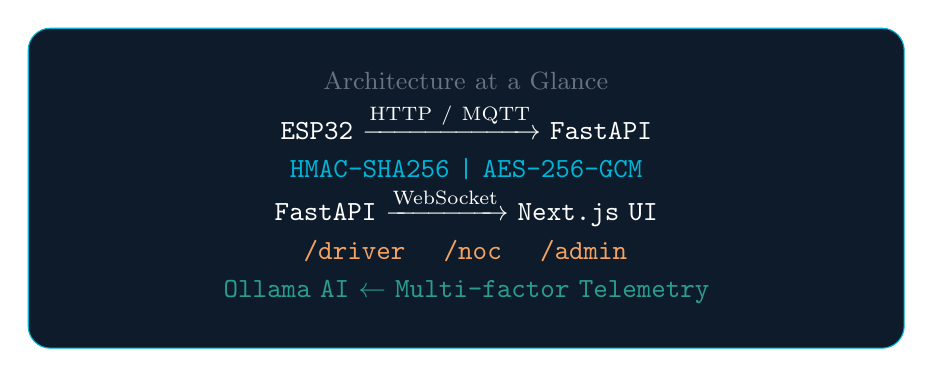
\begin{tikzpicture}
\node[draw=cvisteal,fill=cvisdark,rounded corners=8pt,
      inner sep=16pt,text width=10cm,align=center]{
  {\small\color{cvisgray}Architecture at a Glance}\\[4pt]
  {\color{white}\texttt{ESP32} $\xrightarrow{\text{HTTP / MQTT}}$ \texttt{FastAPI}}\\[2pt]
  {\color{cvisteal}\texttt{HMAC-SHA256 | AES-256-GCM}}\\[2pt]
  {\color{white}\texttt{FastAPI} $\xrightarrow{\text{WebSocket}}$ \texttt{Next.js UI}}\\[2pt]
  {\color{cvisgold}\texttt{/driver \quad /noc \quad /admin}}\\[2pt]
  {\color{cvisgreen}\texttt{Ollama AI} $\leftarrow$ \texttt{Multi-factor Telemetry}}
};
\end{tikzpicture}

\vfill
{\small\color{cvisgray}Generated from live codebase — \today}
\end{titlepage}
\pagecolor{white}
\color{black}

% ═══════════════════════════════════════════════════════════════════════════════
%  TABLE OF CONTENTS
% ═══════════════════════════════════════════════════════════════════════════════
\tableofcontents
\newpage

% ═══════════════════════════════════════════════════════════════════════════════
%  LIST OF TABLES AND FIGURES
% ═══════════════════════════════════════════════════════════════════════════════
\listoftables
\listoffigures
\newpage

% ═══════════════════════════════════════════════════════════════════════════════
%  CHAPTER 1 — PROJECT OVERVIEW
% ═══════════════════════════════════════════════════════════════════════════════
\chapter{Project Overview}

\section{Project Identity}

The \textbf{Connected Vehicle Intelligence System (CVIS)} is an academic prototype built for the \textit{Computer Communication \& Network Security (CCNS)} course. Its central thesis is that AI reasoning belongs in the cloud, not embedded in each vehicle. The vehicle is a \textit{thin, securely-networked client}; the laptop running the backend acts as the data-centre. CVIS demonstrates the \textbf{secure communication layer} that makes this architecture viable.

\begin{ccnsbox}{Core Thesis}
AI lives centrally (cloud/data-centre). The vehicle is a thin client. The project grades the \textbf{secure communication pipeline}, not the AI itself.
\end{ccnsbox}

\section{Core Objectives}
\begin{enumerate}[leftmargin=1.8cm]
  \item Simulate a realistic EV telemetry pipeline from edge device to centralised server.
  \item Enforce cryptographic integrity (HMAC-SHA256) and optional confidentiality (AES-256-GCM) on every packet.
  \item Demonstrate runtime protocol switching between HTTP REST and MQTT publish-subscribe without restarting any service.
  \item Provide a live Network Operations Center (NOC) dashboard that visualises packet flow, security events, and chaos simulations in real time.
  \item Integrate Ollama AI reasoning over multi-factor telemetry to produce contextually accurate driver recommendations.
\end{enumerate}

\section{Non-Goals}
\begin{itemize}
  \item Real EV hardware or real sensors — telemetry is simulated on an ESP32 or via the Python physics engine.
  \item A generic chatbot with no telemetry grounding.
  \item Three separate frontend codebases (one unified Next.js app serves all three roles).
\end{itemize}

% ═══════════════════════════════════════════════════════════════════════════════
%  CHAPTER 2 — SYSTEM ARCHITECTURE
% ═══════════════════════════════════════════════════════════════════════════════
\chapter{System Architecture}

\section{High-Level Architecture Diagram}

\begin{figure}[H]
\centering
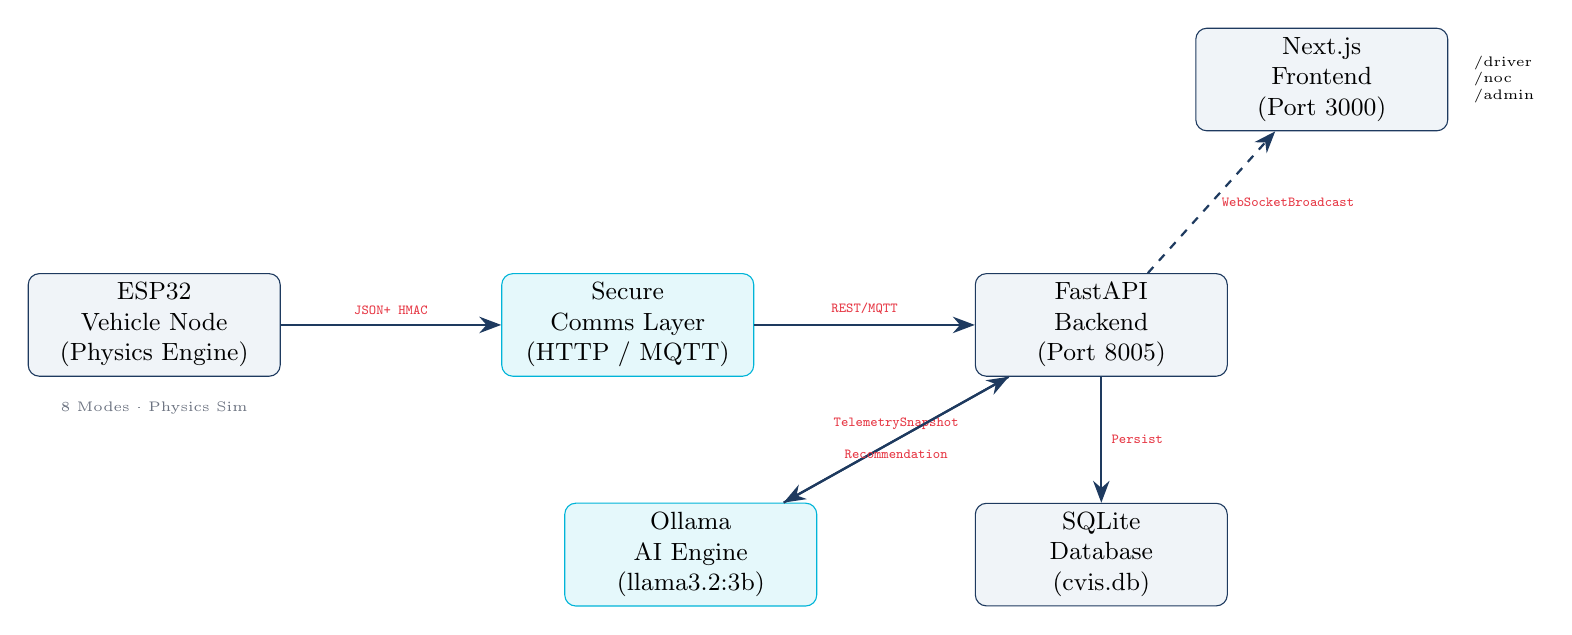
\begin{tikzpicture}[
  node distance=1.8cm and 2.4cm,
  every node/.style={font=\small},
  block/.style={draw=cvisblue, fill=cvislightbg, rounded corners=4pt,
                minimum width=3.2cm, minimum height=1cm, align=center},
  cloud/.style={draw=cvisteal, fill=cvisteal!10, rounded corners=4pt,
                minimum width=3.2cm, minimum height=1cm, align=center},
  arrow/.style={-{Stealth[scale=1.2]}, thick, color=cvisblue},
  label/.style={font=\tiny\ttfamily, color=cvisred}
]

% Row 1 — Edge
\node[block] (esp) {ESP32\\Vehicle Node\\(Physics Engine)};

% Row 2 — Transport
\node[cloud, right=2.8cm of esp] (layer) {Secure\\Comms Layer\\(HTTP / MQTT)};

% Row 3 — Backend
\node[block, right=2.8cm of layer] (fastapi) {FastAPI\\Backend\\(Port 8005)};

% Row 4 — Storage
\node[block, below=1.6cm of fastapi] (sqlite) {SQLite\\Database\\(cvis.db)};

% Row 5 — AI
\node[cloud, left=2cm of sqlite] (ollama) {Ollama\\AI Engine\\(llama3.2:3b)};

% Row 6 — Frontend
\node[block, above=1.8cm of fastapi, xshift=2.8cm] (frontend) {Next.js\\Frontend\\(Port 3000)};

% Connections
\draw[arrow] (esp) -- node[above,label]{JSON\\+ HMAC} (layer);
\draw[arrow] (layer) -- node[above,label]{REST/MQTT} (fastapi);
\draw[arrow] (fastapi) -- node[right,label]{Persist} (sqlite);
\draw[arrow] (fastapi) -- node[above,label]{Telemetry\\Snapshot} (ollama);
\draw[arrow] (ollama) -- node[below,label]{Recommendation} (fastapi);
\draw[arrow,dashed] (fastapi) -- node[right,label]{WebSocket\\Broadcast} (frontend);

% Labels on ESP32
\node[below=0.2cm of esp, font=\tiny, color=cvisgray] {8 Modes · Physics Sim};

% Labels on frontend
\node[right=0.2cm of frontend, align=left, font=\tiny] {
  /driver\\
  /noc\\
  /admin
};

\end{tikzpicture}
\caption{CVIS High-Level System Architecture}
\label{fig:architecture}
\end{figure}

\section{Component Summary}

\begin{table}[H]
\centering
\caption{CVIS Component Inventory}
\label{tab:components}
\begin{tabularx}{\textwidth}{L{2.5cm} L{2.5cm} L{2.5cm} X}
\toprule
\textbf{Component} & \textbf{Technology} & \textbf{Location} & \textbf{Role} \\
\midrule
ESP32 Firmware & Arduino C++ & \texttt{/firmware} & Stateful physics engine; generates telemetry; signs with HMAC; supports HTTP + MQTT \\
Python Simulator & Python 3 & \texttt{/backend/simulator.py} & Local vehicle physics emulator; same logic as firmware, used for development \\
FastAPI Backend & Python + FastAPI & \texttt{/backend} & Core server: auth, crypto, chaos middleware, AI bridge, WebSocket fan-out \\
SQLite Database & aiosqlite & \texttt{/backend/cvis.db} & Persists packets, telemetry, devices, auth logs, and server config \\
Ollama AI & llama3.2:3b / phi3-mini & Local Ollama & Multi-factor telemetry reasoning, driver recommendations, free-text chat \\
Next.js Frontend & Next.js + Tailwind & \texttt{/frontend} & Unified three-role UI: Driver, NOC, Admin \\
\bottomrule
\end{tabularx}
\end{table}

% ═══════════════════════════════════════════════════════════════════════════════
%  CHAPTER 3 — COMMUNICATION LAYER
% ═══════════════════════════════════════════════════════════════════════════════
\chapter{Communication Layer}

\section{Protocol Overview}

CVIS supports two fully-functional transport protocols, switchable at runtime with zero restarts:

\begin{table}[H]
\centering
\caption{Transport Protocol Comparison}
\label{tab:protocols}
\begin{tabularx}{\textwidth}{L{2.8cm} X X}
\toprule
\textbf{Property} & \textbf{HTTP REST} & \textbf{MQTT Pub/Sub} \\
\midrule
Pattern & Request-Response & Publish-Subscribe \\
Connection & Stateless, per-request & Persistent TCP via broker \\
Topic/Endpoint & \texttt{POST /api/v1/telemetry} & \texttt{cvis/telemetry/\{device\_id\}} \\
Auth mechanism & \texttt{X-API-Key} header & \texttt{\_meta.api\_key} in envelope \\
HMAC transport & \texttt{X-HMAC-Signature} header & \texttt{\_meta.hmac} in envelope \\
Config subscribe & Poll \texttt{/api/v1/config/protocol} & Subscribe \texttt{cvis/config/\#} \\
Switch latency & Immediate (next packet) & MQTT broker must be running \\
Best used when & Demonstration, reliability & Bandwidth-constrained, IoT \\
\bottomrule
\end{tabularx}
\end{table}

\section{Packet Flow — HTTP}

\begin{figure}[H]
\centering
\begin{tikzpicture}[
  node distance=0.8cm,
  every node/.style={font=\small},
  step/.style={draw=cvisblue, fill=cvislightbg, rounded corners=3pt,
               minimum width=10cm, minimum height=0.7cm, align=left,
               inner sep=6pt},
  arrow/.style={-{Stealth[scale=1]}, thick, color=cvisteal},
  label/.style={font=\tiny\ttfamily, color=cvisred, right}
]

\node[step] (s1) {\textbf{1.} ESP32 builds JSON payload with all telemetry fields};
\node[step, below=0.3cm of s1] (s2) {\textbf{2.} HMAC-SHA256(device\_secret, raw\_json) → hex signature};
\node[step, below=0.3cm of s2] (s3) {\textbf{3.} [Optional] AES-256-GCM encrypt payload → \{iv, ct, tag\}};
\node[step, below=0.3cm of s3] (s4) {\textbf{4.} HTTP POST /api/v1/telemetry with X-API-Key + X-HMAC-Signature};
\node[step, below=0.3cm of s4] (s5) {\textbf{5.} ChaosMiddleware: apply latency / drop / tamper if configured};
\node[step, below=0.3cm of s5] (s6) {\textbf{6.} auth.py: verify X-API-Key against devices table (SHA-256 hash)};
\node[step, below=0.3cm of s6] (s7) {\textbf{7.} auth.py: verify HMAC-SHA256 signature → reject on mismatch};
\node[step, below=0.3cm of s7] (s8) {\textbf{8.} [If encrypted] AES-GCM decrypt; verify GCM authentication tag};
\node[step, below=0.3cm of s8] (s9) {\textbf{9.} Pydantic validates fields; persist to packets + telemetry tables};
\node[step, below=0.3cm of s9] (s10) {\textbf{10.} WebSocket broadcast to /driver, /noc, /admin frontend views};
\node[step, below=0.3cm of s10] (s11) {\textbf{11.} [Background] Ollama AI analyses snapshot, result broadcast};

\draw[arrow] (s1) -- (s2); \draw[arrow] (s2) -- (s3); \draw[arrow] (s3) -- (s4);
\draw[arrow] (s4) -- (s5); \draw[arrow] (s5) -- (s6); \draw[arrow] (s6) -- (s7);
\draw[arrow] (s7) -- (s8); \draw[arrow] (s8) -- (s9); \draw[arrow] (s9) -- (s10);
\draw[arrow] (s10) -- (s11);

\end{tikzpicture}
\caption{HTTP Telemetry Ingest Pipeline}
\label{fig:http-flow}
\end{figure}

\section{Packet Schema}

Every packet conforms to the following JSON schema (defined in \texttt{backend/models.py}):

\begin{table}[H]
\centering
\caption{Telemetry Payload Schema v1.0}
\label{tab:schema}
\begin{tabularx}{\textwidth}{L{3.5cm} L{2cm} C{1.8cm} X}
\toprule
\textbf{Field} & \textbf{Type} & \textbf{Required} & \textbf{Description \& Bounds} \\
\midrule
\texttt{device\_id} & string & Yes & Unique vehicle ID (1–64 chars) \\
\texttt{schema\_version} & string & No & Schema version, default \texttt{"1.0"} \\
\texttt{timestamp\_ms} & integer & Yes & ESP32 \texttt{millis()} at packet creation \\
\texttt{mode} & string & Yes & One of 8 allowed modes (see Table~\ref{tab:modes}) \\
\texttt{speed\_kmh} & float & No & Vehicle speed; $0 \leq v \leq 250$ km/h \\
\texttt{battery\_pct} & float & No & State of charge; $0 \leq \text{SoC} \leq 100$\% \\
\texttt{battery\_temp\_c} & float & No & Battery pack temp; $-20 \leq T \leq 100$°C \\
\texttt{motor\_temp\_c} & float & No & Motor temp; $-20 \leq T \leq 150$°C \\
\texttt{range\_km} & float & No & Estimated remaining range; $0 \leq r \leq 1000$ km \\
\texttt{fault\_code} & integer & No & \texttt{0x00} = none, \texttt{0x02} = overheat, \texttt{0x04} = motor \\
\texttt{charging\_rate\_w} & float & No & Charging power; 0 when not charging \\
\midrule
\multicolumn{4}{l}{\textit{Advanced Physics Fields (Optional — Schema v2.3)}} \\
\midrule
\texttt{ambient\_temp\_c} & float & No & Outside air temperature in °C \\
\texttt{headwind\_kmh} & float & No & Headwind speed in km/h \\
\texttt{road\_gradient\_pct} & float & No & Road gradient (+uphill / −downhill) \\
\texttt{tire\_pressure\_psi} & float & No & Average tire pressure in PSI \\
\texttt{cabin\_climate\_w} & float & No & AC/Heater power draw in Watts \\
\texttt{max\_cell\_voltage\_delta} & float & No & Max voltage difference between cells (V) \\
\bottomrule
\end{tabularx}
\end{table}

% ═══════════════════════════════════════════════════════════════════════════════
%  CHAPTER 4 — SECURITY IMPLEMENTATION
% ═══════════════════════════════════════════════════════════════════════════════
\chapter{Security Implementation}

\section{Security Layer Architecture}

\begin{figure}[H]
\centering
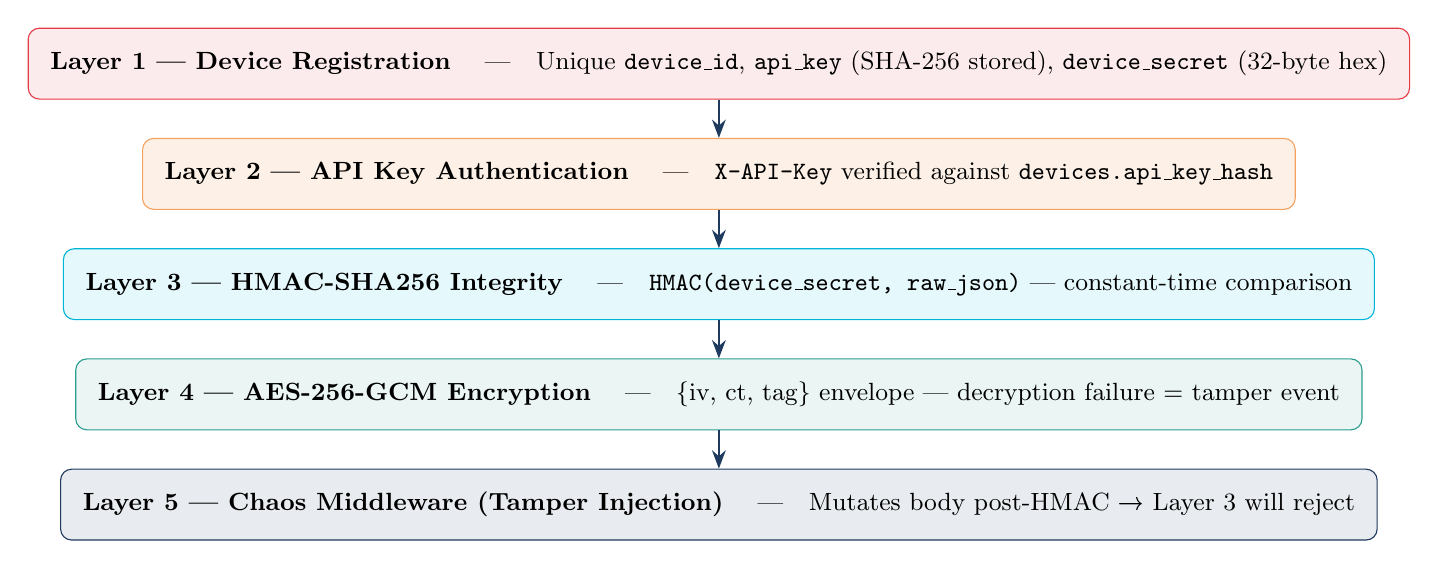
\begin{tikzpicture}[
  every node/.style={font=\small},
  layer/.style={draw=cvisblue, fill=cvislightbg, rounded corners=4pt,
                minimum width=12cm, minimum height=0.9cm, align=center,
                inner sep=8pt},
  arrow/.style={-{Stealth[scale=1]}, thick, color=cvisblue},
  sidebar/.style={font=\tiny\ttfamily, color=cvisgray}
]

\node[layer, fill=cvisred!10, draw=cvisred] (l1) at (0,0)
  {\textbf{Layer 1 — Device Registration} \quad|\quad Unique \texttt{device\_id}, \texttt{api\_key} (SHA-256 stored), \texttt{device\_secret} (32-byte hex)};

\node[layer, fill=cvisgold!15, draw=cvisgold] (l2) at (0,-1.4)
  {\textbf{Layer 2 — API Key Authentication} \quad|\quad \texttt{X-API-Key} verified against \texttt{devices.api\_key\_hash}};

\node[layer, fill=cvisteal!10, draw=cvisteal] (l3) at (0,-2.8)
  {\textbf{Layer 3 — HMAC-SHA256 Integrity} \quad|\quad \texttt{HMAC(device\_secret, raw\_json)} — constant-time comparison};

\node[layer, fill=cvisgreen!10, draw=cvisgreen] (l4) at (0,-4.2)
  {\textbf{Layer 4 — AES-256-GCM Encryption} \quad|\quad \{iv, ct, tag\} envelope — decryption failure = tamper event};

\node[layer, fill=cvisblue!10, draw=cvisblue] (l5) at (0,-5.6)
  {\textbf{Layer 5 — Chaos Middleware (Tamper Injection)} \quad|\quad Mutates body post-HMAC → Layer 3 will reject};

\draw[arrow] (l1) -- (l2); \draw[arrow] (l2) -- (l3); \draw[arrow] (l3) -- (l4); \draw[arrow] (l4) -- (l5);

\end{tikzpicture}
\caption{CVIS Security Layer Stack}
\label{fig:security}
\end{figure}

\section{Device Registration Flow}

When the Python simulator or an ESP32 first connects:

\begin{enumerate}
  \item \texttt{POST /api/v1/devices/register} with \texttt{\{"device\_id": "SIM-001"\}}.
  \item Backend generates: \texttt{api\_key = secrets.token\_hex(32)} and \texttt{device\_secret = secrets.token\_hex(32)}.
  \item \texttt{api\_key\_hash = SHA256(api\_key)} is stored in \texttt{devices} table. The plaintext \texttt{api\_key} is returned once.
  \item All subsequent requests include \texttt{X-API-Key: <plaintext>} and \texttt{X-HMAC-Signature: <hex>}.
\end{enumerate}

\section{HMAC-SHA256 Implementation}

HMAC is computed over the \textit{exact raw JSON bytes} as transmitted. This is critical: even a single extra space in the JSON would change the HMAC and trigger rejection.

\begin{lstlisting}[language=Python, caption=HMAC Computation (backend/crypto.py)]
def compute_hmac(secret_hex: str, payload: str) -> str:
    key = bytes.fromhex(secret_hex)        # 32-byte (256-bit) key
    sig = hmac.new(key, payload.encode("utf-8"), hashlib.sha256)
    return sig.hexdigest()                 # 64-char lowercase hex

def verify_hmac(secret_hex: str, payload: str, signature_hex: str) -> bool:
    expected = compute_hmac(secret_hex, payload)
    # hmac.compare_digest prevents timing-oracle attacks
    return hmac.compare_digest(expected, signature_hex.strip().lower())
\end{lstlisting}

\section{AES-256-GCM Encryption}

\begin{lstlisting}[language=Python, caption=AES-GCM Encrypt/Decrypt (backend/crypto.py)]
def aes_gcm_encrypt(secret_hex: str, plaintext: str) -> dict:
    key    = bytes.fromhex(secret_hex)   # 32 bytes = 256-bit AES key
    aesgcm = AESGCM(key)
    nonce  = os.urandom(12)              # 96-bit random nonce per message
    ct_with_tag = aesgcm.encrypt(nonce, plaintext.encode("utf-8"), None)
    ct  = ct_with_tag[:-16]             # ciphertext bytes
    tag = ct_with_tag[-16:]             # 128-bit GCM authentication tag
    return {"iv": nonce.hex(), "ct": ct.hex(), "tag": tag.hex()}
\end{lstlisting}

The GCM \textbf{authentication tag} doubles as an integrity check: decrypting with a mismatched key or tampered ciphertext raises \texttt{InvalidTag}, which the backend logs as a \texttt{tamper\_detected} event.

\section{Fault Codes}

\begin{table}[H]
\centering
\caption{Vehicle Fault Codes}
\label{tab:faults}
\begin{tabularx}{\textwidth}{C{2cm} L{3.5cm} X}
\toprule
\textbf{Code (hex)} & \textbf{Name} & \textbf{Description \& Physics Trigger} \\
\midrule
\texttt{0x00} & No Fault & Normal operation \\
\texttt{0x02} & Battery Overheating & Battery temp > 60°C — caused by high discharge rate under load \\
\texttt{0x04} & Motor Fault & Motor temp > 95°C — caused by high speed + uphill gradient + drag \\
\bottomrule
\end{tabularx}
\end{table}

% ═══════════════════════════════════════════════════════════════════════════════
%  CHAPTER 5 — VEHICLE SIMULATION ENGINE
% ═══════════════════════════════════════════════════════════════════════════════
\chapter{Vehicle Simulation Engine}

\section{Physics Model Overview}

The simulator is a \textbf{stateful physics engine}. Each tick (every 2 seconds) computes the next state based on the current state. No values are hardcoded per mode; modes are \textit{emergent} from the physics.

\subsection{Load Factor Computation}

The \textbf{Load Factor} ($L$) is the normalised measure of how hard the vehicle is working at any instant:

\begin{equation}
L = \underbrace{\frac{v}{50}}_{\text{speed drag}} + \underbrace{\frac{(v + w)^2}{10000}}_{\text{aerodynamic drag}} + \underbrace{g \cdot 0.5}_{\text{gravity drag}} + \underbrace{\max\!\left(0,\; \frac{36 - p_t}{10}\right)}_{\text{tire drag}}
\label{eq:load}
\end{equation}

where $v$ = speed (km/h), $w$ = headwind (km/h), $g$ = road gradient (\%), $p_t$ = tire pressure (PSI).

\subsection{Battery Drain Model}

\begin{equation}
\Delta \text{SoC} = \left(L \cdot 0.1 + \frac{P_{\text{cabin}}}{5000}\right) \cdot \Delta t
\label{eq:drain}
\end{equation}

\subsection{Thermal Model}

\textbf{Motor Temperature:}
\begin{equation}
\Delta T_{\text{motor}} = (L \cdot 2.0 - (T_{\text{motor}} - T_{\text{ambient}}) \cdot 0.05) \cdot \Delta t
\label{eq:motor-temp}
\end{equation}

\textbf{Battery Temperature:}
\begin{equation}
\Delta T_{\text{battery}} = (\Delta \text{SoC} \cdot 5.0 - (T_{\text{battery}} - T_{\text{ambient}}) \cdot 0.02) \cdot \Delta t
\label{eq:batt-temp}
\end{equation}

\subsection{Range Estimation}

\begin{equation}
r = \text{SoC} \times 3.0 \times f_{\text{tire}} \times f_{\text{wind}} \times f_{\text{cabin}}
\label{eq:range}
\end{equation}

where penalty factors are: $f_{\text{tire}} = 0.9$ if $p_t < 32\;\text{PSI}$; $f_{\text{wind}} = 0.85$ if $w > 20\;\text{km/h}$; $f_{\text{cabin}} = 0.95$ if $P_{\text{cabin}} > 1000\;\text{W}$.

\section{Vehicle Operating Modes}

\begin{table}[H]
\centering
\caption{Vehicle Operating Modes — Emergent Classification}
\label{tab:modes}
\begin{tabularx}{\textwidth}{L{3.8cm} L{2.8cm} X}
\toprule
\textbf{Mode} & \textbf{Classification Trigger} & \textbf{Typical Characteristics} \\
\midrule
Healthy & $30 \leq v \leq 80$ km/h & Normal cruise; moderate load \\
Eco & (button-selected / low speed) & Conservative speed, max range \\
Sport & $v > 80$ km/h & High motor temp, fast drain \\
Heavy Traffic & $0 < v < 30$ km/h & Stop-start, cabin AC dominant \\
Low Battery & SoC $\leq 15$\% & Speed limited; urgent AI alert \\
Battery Overheating & $T_{\text{batt}} > 60$°C & Fault 0x02; limp mode (40 km/h cap) \\
Charging & $v = 0$ and $P_{\text{charge}} > 0$ & Battery replenishing \\
Motor Fault & $T_{\text{motor}} > 95$°C & Fault 0x04; forced stop \\
\bottomrule
\end{tabularx}
\end{table}

\section{Physics Interdependency Map}

\begin{figure}[H]
\centering
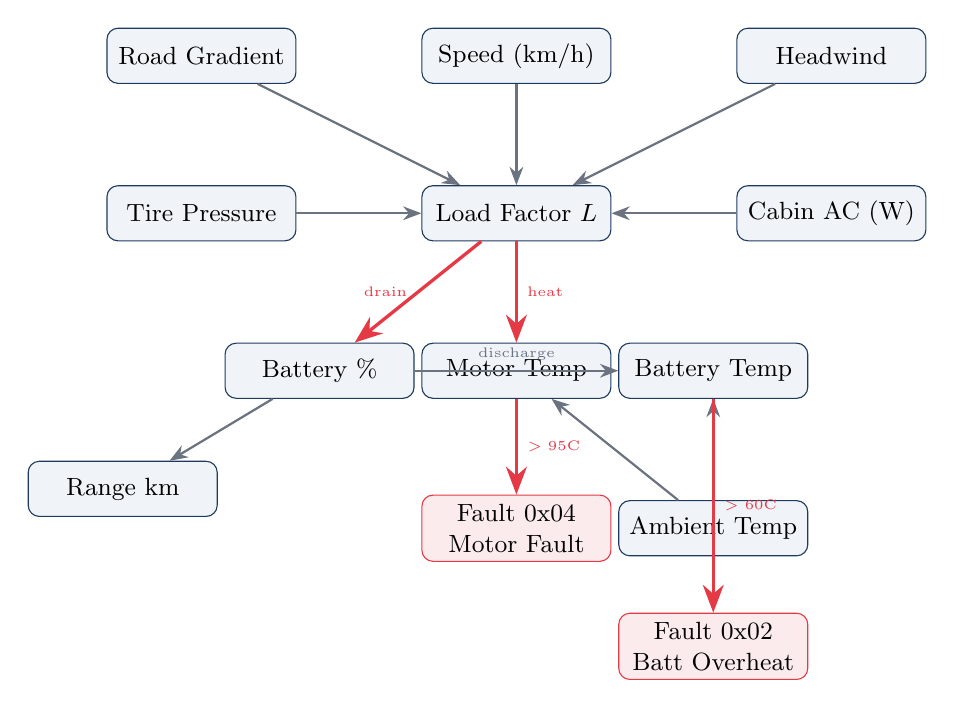
\begin{tikzpicture}[
  every node/.style={font=\small},
  var/.style={draw=cvisblue, fill=cvislightbg, rounded corners=4pt,
              minimum width=2.4cm, minimum height=0.7cm, align=center},
  fault/.style={draw=cvisred, fill=cvisred!10, rounded corners=4pt,
                minimum width=2.4cm, minimum height=0.7cm, align=center},
  cause/.style={-{Stealth[scale=1.0]}, thick, color=cvisgray},
  strong/.style={-{Stealth[scale=1.2]}, very thick, color=cvisred},
]

\node[var] (speed)   at (0,0)       {Speed (km/h)};
\node[var] (grad)    at (-4,0)      {Road Gradient};
\node[var] (wind)    at (4,0)       {Headwind};
\node[var] (tire)    at (-4,-2)     {Tire Pressure};
\node[var] (cabin)   at (4,-2)      {Cabin AC (W)};
\node[var] (load)    at (0,-2)      {Load Factor $L$};
\node[var] (battery) at (-2.5,-4)   {Battery \%};
\node[var] (batt_t)  at (2.5,-4)    {Battery Temp};
\node[var] (motor_t) at (0,-4)      {Motor Temp};
\node[var] (range)   at (-5,-5.5)   {Range km};
\node[var] (ambient) at (2.5,-6)    {Ambient Temp};
\node[fault] (f02)   at (2.5,-7.5)  {Fault 0x02\\Batt Overheat};
\node[fault] (f04)   at (0,-6)      {Fault 0x04\\Motor Fault};

\draw[cause] (speed) -- (load);
\draw[cause] (grad) -- (load);
\draw[cause] (wind) -- (load);
\draw[cause] (tire) -- (load);
\draw[cause] (cabin) -- (load);
\draw[strong] (load) -- (battery)  node[midway,left,font=\tiny]{drain};
\draw[strong] (load) -- (motor_t)  node[midway,right,font=\tiny]{heat};
\draw[cause] (battery) -- (batt_t) node[midway,above,font=\tiny]{discharge};
\draw[cause] (battery) -- (range);
\draw[cause] (ambient) -- (motor_t);
\draw[cause] (ambient) -- (batt_t);
\draw[strong] (motor_t) -- (f04)   node[midway,right,font=\tiny]{$>95°$C};
\draw[strong] (batt_t) -- (f02)    node[midway,right,font=\tiny]{$>60°$C};

\end{tikzpicture}
\caption{Physics Variable Interdependency Graph}
\label{fig:physics}
\end{figure}

% ═══════════════════════════════════════════════════════════════════════════════
%  CHAPTER 6 — AI INTEGRATION
% ═══════════════════════════════════════════════════════════════════════════════
\chapter{AI Integration}

\section{Architecture}

CVIS uses \textbf{Ollama} running locally with \texttt{llama3.2:3b} (or \texttt{phi3-mini}). The AI is called via HTTP to \texttt{http://localhost:11434/api/chat}. The model is never called directly from the frontend — it is always mediated by the FastAPI backend, which ensures telemetry grounding.

\section{Two AI Surfaces}

\begin{table}[H]
\centering
\caption{AI Endpoints}
\label{tab:ai}
\begin{tabularx}{\textwidth}{L{3.5cm} L{3.5cm} X}
\toprule
\textbf{Surface} & \textbf{Endpoint} & \textbf{Behaviour} \\
\midrule
Auto Recommendation & Background task per telemetry update & Analyses combined snapshot; produces severity-tagged alert; broadcast via WebSocket \\
Driver Chat & \texttt{POST /api/v1/ai/chat} & Free-text Q\&A grounded in current + last 10 readings; cannot invent vehicle state \\
\bottomrule
\end{tabularx}
\end{table}

\section{Prompt Engineering}

The prompt is built in \texttt{backend/ai/prompt\_builder.py}. The user message sent to Ollama contains:

\begin{enumerate}
  \item \textbf{Current Snapshot}: all 17 telemetry fields from the latest packet.
  \item \textbf{Advanced Physics Section}: ambient temp, headwind, road gradient, tire pressure, cabin load, cell voltage delta — labelled \texttt{=== ADVANCED PHYSICS ===}.
  \item \textbf{Trend Block}: last 5 readings rendered as a sparkline text table (battery \%, speed, motor temp, mode).
  \item \textbf{Range Violations}: any field that has crossed its warning threshold.
  \item \textbf{Mode Transition}: previous mode is explicitly shown when a mode change is detected.
\end{enumerate}

The system prompt instructs the model to: (1) classify severity as \texttt{NORMAL/CAUTION/WARNING/CRITICAL}, (2) reason from the \textit{combination} of factors rather than any single threshold, and (3) output exactly two lines: severity label + recommendation.

\section{AI Throttling}

To prevent LLM overload, the background AI task fires only when:
\begin{itemize}
  \item At least 20 seconds have elapsed since the last inference, \textbf{OR}
  \item The vehicle mode has changed since the last packet.
\end{itemize}

% ═══════════════════════════════════════════════════════════════════════════════
%  CHAPTER 7 — DATABASE SCHEMA
% ═══════════════════════════════════════════════════════════════════════════════
\chapter{Database Schema}

\section{Schema Overview}

All data is persisted in a single SQLite file (\texttt{backend/cvis.db}) using \texttt{aiosqlite} for non-blocking async access. The schema uses WAL (Write-Ahead Logging) for concurrent read-write.

\begin{table}[H]
\centering
\caption{Database Tables}
\label{tab:db}
\begin{tabularx}{\textwidth}{L{3cm} L{3cm} X}
\toprule
\textbf{Table} & \textbf{Primary Key} & \textbf{Purpose} \\
\midrule
\texttt{packets} & \texttt{id} (auto) & Raw log of every inbound packet; protocol-agnostic \\
\texttt{telemetry} & \texttt{id} (auto) & Parsed, structured telemetry fields per packet \\
\texttt{devices} & \texttt{device\_id} & Registered vehicle nodes with API key hash and secret \\
\texttt{auth\_logs} & \texttt{id} (auto) & Every auth and tamper event \\
\texttt{server\_config} & \texttt{key} & Key-value store for all runtime configuration \\
\texttt{schema\_version} & \texttt{version} & Migration history tracker \\
\bottomrule
\end{tabularx}
\end{table}

\section{Packets Table}

\begin{lstlisting}[language=SQL, caption=Packets Table DDL]
CREATE TABLE packets (
    id                INTEGER PRIMARY KEY AUTOINCREMENT,
    received_at       TEXT    NOT NULL,
    device_id         TEXT    NOT NULL,
    protocol          TEXT    NOT NULL DEFAULT 'http',  -- 'http' | 'mqtt'
    direction         TEXT    NOT NULL DEFAULT 'inbound',
    size_bytes        INTEGER,
    status            TEXT    NOT NULL,    -- 'ok' | 'tamper_detected' | ...
    raw_json          TEXT    NOT NULL,
    encrypted         INTEGER NOT NULL DEFAULT 0,       -- 0 | 1
    encryption_method TEXT    NOT NULL DEFAULT 'PLAIN', -- 'PLAIN' | 'AES-GCM'
    auth_status       TEXT    NOT NULL DEFAULT 'ok'
);
\end{lstlisting}

\section{Server Config Keys}

\begin{table}[H]
\centering
\caption{Runtime Server Configuration Keys}
\label{tab:config}
\begin{tabularx}{\textwidth}{L{4cm} L{2.5cm} X}
\toprule
\textbf{Key} & \textbf{Default} & \textbf{Description} \\
\midrule
\texttt{active\_protocol} & \texttt{http} & Current transport protocol (\texttt{http}/\texttt{mqtt}) \\
\texttt{encryption\_enabled} & \texttt{false} & AES-256-GCM toggle \\
\texttt{auth\_enabled} & \texttt{true} & API key + HMAC enforcement toggle \\
\texttt{replay\_protection} & \texttt{false} & Timestamp-window replay protection \\
\texttt{chaos\_loss\_pct} & \texttt{0} & Packet loss rate (0/5/10/25\%) \\
\texttt{chaos\_latency\_ms} & \texttt{0} & Artificial latency (0/100/300/1000 ms) \\
\texttt{chaos\_tamper} & \texttt{false} & Payload mutation injector \\
\texttt{mobile\_app\_enabled} & \texttt{true} & Global mobile access gate \\
\texttt{force\_mode} & \texttt{""} & Override vehicle simulation mode \\
\bottomrule
\end{tabularx}
\end{table}

% ═══════════════════════════════════════════════════════════════════════════════
%  CHAPTER 8 — NETWORK OPERATIONS CENTER (NOC)
% ═══════════════════════════════════════════════════════════════════════════════
\chapter{Network Operations Center (NOC)}

\section{NOC Purpose}

The NOC at \texttt{/noc} is the centrepiece of the CVIS demonstration. It visualises every network event in real time and provides live controls that each trigger a \textit{verifiable backend behaviour change}. No toggle is cosmetic.

\section{NOC Terminology Glossary}

\begin{table}[H]
\centering
\caption{NOC Terminology Reference}
\label{tab:terminology}
\begin{tabularx}{\textwidth}{L{4cm} X}
\toprule
\textbf{Term} & \textbf{Definition} \\
\midrule
\textbf{Packet} & A single JSON payload from one vehicle tick, transported via HTTP POST or MQTT PUBLISH \\
\textbf{RTT (Round-Trip Time)} & Time from packet dispatch to acknowledgement receipt — artificially elevated by the Latency slider \\
\textbf{HMAC} & Hash-based Message Authentication Code — proves the payload was not modified in transit \\
\textbf{AES-GCM} & Advanced Encryption Standard in Galois/Counter Mode — provides both confidentiality and integrity \\
\textbf{Auth Status} & \texttt{auth\_ok} | \texttt{auth\_fail} | \texttt{no\_auth} | \texttt{tamper\_detected} \\
\textbf{Encryption Status} & \texttt{PLAIN} (unencrypted) or \texttt{AES-GCM} (encrypted envelope) \\
\textbf{Packet Loss \%} & Percentage of packets randomly dropped by the ChaosMiddleware before processing \\
\textbf{Chaos Latency} & Synthetic delay injected per packet in the middleware \\
\textbf{Tamper Injection} & Mutates a payload field \textit{after} HMAC is computed, guaranteeing the backend rejects it \\
\textbf{Protocol Switch} & Live toggle between HTTP REST and MQTT; the backend broadcasts the change via MQTT so ESP32 nodes self-switch \\
\textbf{Replay Attack} & Re-sending an old captured packet to trick the backend — countered by timestamp-window protection \\
\textbf{Limp Mode} & Battery Overheating fault state: speed capped at 40 km/h by physics engine \\
\textbf{Fan-out} & One WebSocket broadcast from backend reaches \textit{all} connected frontend tabs simultaneously \\
\bottomrule
\end{tabularx}
\end{table}

\section{NOC Live Controls}

\begin{table}[H]
\centering
\caption{NOC Live Controls — Backend Effect Mapping}
\label{tab:controls}
\begin{tabularx}{\textwidth}{L{3.5cm} L{4cm} X}
\toprule
\textbf{Control} & \textbf{API Endpoint} & \textbf{Real Backend Effect} \\
\midrule
Protocol Switch & \texttt{POST /api/v1/config/protocol} & Changes \texttt{active\_protocol} in DB; broadcasts to MQTT \texttt{cvis/config/protocol}; ESP32 self-switches on next poll \\
Encryption Toggle & \texttt{POST /api/v1/config/encryption} & Toggles AES-GCM; broadcasts to MQTT; ESP32 switches payload format on next packet \\
Auth Toggle & \texttt{POST /api/v1/config/auth} & Enables/disables API key + HMAC verification; traffic accepted without credentials in OFF mode \\
Packet Loss Slider & \texttt{POST /api/v1/config/chaos} & ChaosMiddleware probabilistically returns HTTP 503 before any processing \\
Latency Slider & \texttt{POST /api/v1/config/chaos} & \texttt{asyncio.sleep(latency\_ms)} added before handler runs \\
Tamper Injector & \texttt{POST /api/v1/config/chaos} & Mutates \texttt{battery\_pct=999.9} post-signature; next HMAC check will fail \\
Replay Protection & \texttt{POST /api/v1/config/replay} & Enables timestamp-window deduplication; duplicate packets rejected \\
Disconnect Vehicle & \texttt{POST /api/v1/control/disconnect} & Marks device inactive in DB; future packets from that device rejected \\
Stop AI Service & \texttt{POST /api/v1/control/ai} & Disables background AI task; recommendations paused globally \\
\bottomrule
\end{tabularx}
\end{table}

\section{NOC Packet Inspector Fields}

Each row in the NOC packet table can be expanded to reveal:

\begin{itemize}
  \item \textbf{Packet ID} — sequential integer from \texttt{packets.id}
  \item \textbf{Source / Destination} — device ID → backend IP
  \item \textbf{Timestamp} — ISO 8601, backend receipt time
  \item \textbf{Protocol} — \texttt{http} or \texttt{mqtt}
  \item \textbf{Size (bytes)} — raw JSON body length
  \item \textbf{Auth Status} — \texttt{auth\_ok / auth\_fail / no\_auth / tamper\_detected}
  \item \textbf{Encryption} — \texttt{PLAIN} or \texttt{AES-GCM}
  \item \textbf{Fault Code} — hex fault from telemetry
  \item \textbf{AI Response} — last recommendation generated for this device
  \item \textbf{Raw JSON Payload} — full telemetry JSON (collapsible)
\end{itemize}

% ═══════════════════════════════════════════════════════════════════════════════
%  CHAPTER 9 — FRONTEND PAGES
% ═══════════════════════════════════════════════════════════════════════════════
\chapter{Frontend Pages}

\section{Routing Architecture}

The unified Next.js application (port 3000) provides:

\begin{table}[H]
\centering
\caption{Frontend Routes}
\label{tab:routes}
\begin{tabularx}{\textwidth}{L{3.5cm} L{2.5cm} X}
\toprule
\textbf{URL} & \textbf{Role} & \textbf{Primary Purpose} \\
\midrule
\texttt{/} & Landing & Role selector, project overview \\
\texttt{/driver} & Driver & Live vehicle telemetry, AI chat, health gauges, historical graphs \\
\texttt{/noc} & NOC Engineer & Live packet flow, control panel, security events \\
\texttt{/admin} & Administrator & System stats, auth logs, device registry, server health \\
\texttt{/alphamobile} & Premium Driver & Mobile view for ESP32-ALPHA (Premium tier) \\
\texttt{/betamobile} & Premium Driver & Mobile view for ESP32-BETA (Premium tier) \\
\texttt{/gammamobile} & Free Driver & Mobile view for ESP32-GAMMA (Free tier — gated) \\
\texttt{/deltamobile} & Free Driver & Mobile view for ESP32-DELTA (Free tier — gated) \\
\bottomrule
\end{tabularx}
\end{table}

\section{Driver Dashboard (\texttt{/driver})}

\begin{ccnsbox}{Key Features}
\begin{itemize}[nosep]
  \item Live telemetry gauges: speed, battery SoC, battery temp, motor temp, range, fault code
  \item Operating mode badge with colour coding
  \item AI Recommendation panel (severity-tagged: NORMAL / CAUTION / WARNING / CRITICAL)
  \item Historical trend graphs (Recharts library): battery\%, motor temp, speed over time
  \item Driver Chat: free-text conversation grounded in live telemetry
  \item Active alerts panel driven by WebSocket events
\end{itemize}
\end{ccnsbox}

Data flow: WebSocket \texttt{wss://api-cvis.justinsaju.me/ws} → \texttt{event: telemetry} message → React state update → re-render gauges.

\section{NOC Dashboard (\texttt{/noc})}

\begin{ccnsbox}{Key Features}
\begin{itemize}[nosep]
  \item Live animated packet flow diagram (ESP32 → Backend, colour-coded by protocol and security status)
  \item Packet table with 10 columns: ID, source, dest, timestamp, protocol, size, auth, encryption, fault, RTT
  \item Click-to-expand packet inspector (full JSON payload + AI response)
  \item All 9 live controls wired to real backend endpoints (Table~\ref{tab:controls})
  \item Live chaos metrics: total requests, dropped packets, tampered packets
\end{itemize}
\end{ccnsbox}

\section{Admin Console (\texttt{/admin})}

\begin{ccnsbox}{Key Features}
\begin{itemize}[nosep]
  \item Connected vehicles list with status, tier, and last seen
  \item Server status: uptime, WebSocket client count, AI service health
  \item Packet statistics chart (last 12 hours by protocol)
  \item Auth log table: event type, device, IP, timestamp, details
  \item Failed request tracker and error log
  \item CPU/memory usage indicators
\end{itemize}
\end{ccnsbox}

\section{Mobile Views (\texttt{/alphamobile}, \texttt{/betamobile}, etc.)}

Premium-tier vehicles (ESP32-ALPHA, ESP32-BETA) have a mobile-optimised view accessible at \texttt{/alphamobile} and \texttt{/betamobile}. Free-tier vehicles (GAMMA, DELTA) see a \textit{gated} page. Access is controlled by the NOC's \textbf{Global Mobile App} toggle (\texttt{server\_config.mobile\_app\_enabled}), which is verified server-side per device tier before granting access.

% ═══════════════════════════════════════════════════════════════════════════════
%  CHAPTER 10 — CHAOS / SIMULATION MIDDLEWARE
% ═══════════════════════════════════════════════════════════════════════════════
\chapter{Chaos \& Simulation Middleware}

\section{Purpose}

The \texttt{ChaosMiddleware} (in \texttt{backend/middleware/chaos.py}) simulates adverse network conditions at the \textbf{application middleware layer} rather than at the OS/network level. This is pedagogically equivalent and far simpler to set up in a demo environment.

\section{Middleware Pipeline}

\begin{figure}[H]
\centering
\begin{tikzpicture}[
  every node/.style={font=\small},
  step/.style={draw=cvisblue, fill=cvislightbg, rounded corners=3pt,
               minimum width=9cm, minimum height=0.65cm, align=left,
               inner sep=6pt},
  drop/.style={draw=cvisred, fill=cvisred!10, rounded corners=3pt,
               minimum width=9cm, minimum height=0.65cm, align=left,
               inner sep=6pt},
  arrow/.style={-{Stealth[scale=1]}, thick, color=cvisteal},
]

\node[step] (r1) {\textbf{1.} Read full request body bytes (required for tamper + pass-through)};
\node[step, below=0.25cm of r1] (r2) {\textbf{2.} Artificial latency: \texttt{asyncio.sleep(latency\_ms / 1000)}};
\node[drop, below=0.25cm of r2] (r3) {\textbf{3.} Packet loss: if \texttt{random(1,100) <= loss\_pct} → return HTTP 503};
\node[step, below=0.25cm of r3] (r4) {\textbf{4.} Tamper injection: mutate \texttt{battery\_pct = 999.9} in body JSON};
\node[step, below=0.25cm of r4] (r5) {\textbf{5.} Rebuild \texttt{receive()} callable with (possibly mutated) body};
\node[step, below=0.25cm of r5] (r6) {\textbf{6.} Call \texttt{app(scope, patched\_receive, send)} → normal handler continues};

\draw[arrow] (r1) -- (r2); \draw[arrow] (r2) -- (r3); \draw[arrow] (r3) -- (r4);
\draw[arrow] (r4) -- (r5); \draw[arrow] (r5) -- (r6);

\end{tikzpicture}
\caption{ChaosMiddleware Execution Pipeline}
\label{fig:chaos}
\end{figure}

\section{Tamper Detection Sequence}

When \textbf{tamper injection} is enabled and \textbf{auth is enabled}:

\begin{enumerate}
  \item ESP32 sends JSON with HMAC over the \textit{original} payload.
  \item ChaosMiddleware changes \texttt{battery\_pct: 999.9} in the body.
  \item \texttt{auth.py} reads the (now mutated) body and recomputes HMAC.
  \item HMAC mismatch detected → \texttt{tamper\_detected} event logged to \texttt{auth\_logs}.
  \item Backend returns \texttt{HTTP 401} with \texttt{"HMAC signature verification failed"}.
  \item NOC packet table shows \texttt{auth\_status = tamper\_detected} in red.
\end{enumerate}

% ═══════════════════════════════════════════════════════════════════════════════
%  CHAPTER 11 — API REFERENCE
% ═══════════════════════════════════════════════════════════════════════════════
\chapter{API Reference}

\section{Complete Endpoint Inventory}

\begin{longtable}{L{4.5cm} L{1.8cm} X}
\caption{Full API Endpoint Reference} \label{tab:api} \\
\toprule
\textbf{Endpoint} & \textbf{Method} & \textbf{Description} \\
\midrule
\endfirsthead
\multicolumn{3}{c}{\textit{(Continued from previous page)}} \\
\toprule
\textbf{Endpoint} & \textbf{Method} & \textbf{Description} \\
\midrule
\endhead
\midrule
\multicolumn{3}{r}{\textit{(Continued on next page)}} \\
\endfoot
\bottomrule
\endlastfoot

\multicolumn{3}{l}{\textbf{Telemetry}} \\
\texttt{/api/v1/telemetry} & POST & Ingest telemetry packet (HTTP); requires X-API-Key + X-HMAC-Signature \\
\texttt{/api/v1/telemetry/recent} & GET & Fetch N most recent telemetry rows; optional \texttt{device\_id} filter \\
\texttt{/api/v1/telemetry/packets} & GET & Fetch raw packet log for NOC table \\
\midrule
\multicolumn{3}{l}{\textbf{Devices}} \\
\texttt{/api/v1/devices/register} & POST & Register new device; returns api\_key + device\_secret \\
\texttt{/api/v1/admin/deactivate-device} & POST & Mark device as inactive \\
\midrule
\multicolumn{3}{l}{\textbf{Configuration (NOC Controls)}} \\
\texttt{/api/v1/config/protocol} & GET/POST & Get/set active protocol (http/mqtt) \\
\texttt{/api/v1/config/encryption} & GET/POST & Get/toggle AES-GCM encryption \\
\texttt{/api/v1/config/auth} & GET/POST & Get/toggle API key + HMAC enforcement \\
\texttt{/api/v1/config/chaos} & GET/POST & Get/update packet loss, latency, tamper settings \\
\texttt{/api/v1/config/replay} & GET/POST & Get/toggle timestamp replay protection \\
\texttt{/api/v1/config/all} & GET & Full config snapshot (all settings in one call) \\
\texttt{/api/v1/config/mode} & POST & Force a specific vehicle simulation mode \\
\texttt{/api/v1/config/mobile-access} & GET & Get mobile access state for a vehicle \\
\texttt{/api/v1/config/mobile-app} & POST & Globally enable/disable mobile app access \\
\midrule
\multicolumn{3}{l}{\textbf{AI}} \\
\texttt{/api/v1/ai/recommendation} & POST & On-demand AI recommendation for latest telemetry \\
\texttt{/api/v1/ai/chat} & POST & Driver chat grounded in current + historical telemetry \\
\texttt{/api/v1/ai/status} & GET & Check Ollama availability and model status \\
\midrule
\multicolumn{3}{l}{\textbf{Admin}} \\
\texttt{/api/v1/admin/stats} & GET & System stats: uptime, packet counts, auth counts \\
\texttt{/api/v1/admin/devices} & GET & Connected vehicle list with status and tier \\
\texttt{/api/v1/admin/packet-stats} & GET & Packet statistics over last N hours \\
\texttt{/api/v1/admin/auth-logs} & GET & Authentication and tamper event log \\
\midrule
\multicolumn{3}{l}{\textbf{Control}} \\
\texttt{/api/v1/control/vehicles} & GET & List all vehicles with real-time status \\
\texttt{/api/v1/control/disconnect} & POST & Disconnect / deactivate a vehicle \\
\texttt{/api/v1/control/ai} & POST & Enable/disable AI service globally \\
\midrule
\multicolumn{3}{l}{\textbf{WebSocket \& System}} \\
\texttt{/ws} & WS & WebSocket endpoint; fan-out broadcast to all connected clients \\
\texttt{/health} & GET & Backend health check \\
\texttt{/docs} & GET & Swagger UI auto-generated API docs \\

\end{longtable}

% ═══════════════════════════════════════════════════════════════════════════════
%  CHAPTER 12 — CCNS SYLLABUS MAPPING
% ═══════════════════════════════════════════════════════════════════════════════
\chapter{CCNS Syllabus Mapping}

\begin{longtable}{L{2cm} L{4.5cm} L{4cm} X}
\caption{CVIS Features Mapped to CCNS Units} \label{tab:ccns} \\
\toprule
\textbf{Unit} & \textbf{Topic} & \textbf{CVIS Feature} & \textbf{Where in Code} \\
\midrule
\endfirsthead
\toprule
\textbf{Unit} & \textbf{Topic} & \textbf{CVIS Feature} & \textbf{Where in Code} \\
\midrule
\endhead
\midrule
\endfoot
\bottomrule
\endlastfoot

Unit 1 & Network Topologies, Client-Server & ESP32 (thin client) → FastAPI (server); NOC, Admin, Driver roles & \texttt{main.py}, \texttt{ws\_manager.py} \\
\midrule
Unit 2 & Application Layer Protocols, REST, MQTT Pub/Sub & HTTP REST + MQTT runtime-switchable; MQTT topics \texttt{cvis/telemetry/\#} and \texttt{cvis/config/\#} & \texttt{comms/mqtt\_adapter.py}, \texttt{routers/config.py} \\
\midrule
Unit 3 & Reliability, RTT, Packet Loss, Latency, Retransmission & ChaosMiddleware: configurable loss, latency, tamper; ESP32 retry with exponential backoff & \texttt{middleware/chaos.py}, \texttt{firmware.ino} \\
\midrule
Unit 4 & Authentication, Integrity, Encryption & API Key Auth, HMAC-SHA256, AES-256-GCM, tamper detection logging & \texttt{auth.py}, \texttt{crypto.py}, \texttt{routers/devices.py} \\
\midrule
Unit 4 & Replay Attack Protection & Timestamp-window deduplication; same \texttt{(device\_id, timestamp\_ms)} rejected within window & \texttt{replay\_protection.py}, \texttt{routers/config.py} \\
\midrule
Unit 5 & Cloud/Edge AI, Intelligent Networking & Ollama AI centralised on server; multi-factor reasoning; not embedded per-vehicle & \texttt{ai/ollama\_client.py}, \texttt{ai/prompt\_builder.py} \\
\midrule
Unit 5 & Real-time Data Streaming & WebSocket fan-out; single broadcast reaches all three frontend views simultaneously & \texttt{ws\_manager.py}, \texttt{routers/ws.py} \\

\end{longtable}

% ═══════════════════════════════════════════════════════════════════════════════
%  CHAPTER 13 — STARTUP \& DEPLOYMENT
% ═══════════════════════════════════════════════════════════════════════════════
\chapter{Startup \& Deployment}

\section{Prerequisites}

\begin{table}[H]
\centering
\caption{Software Prerequisites}
\label{tab:prereqs}
\begin{tabularx}{\textwidth}{L{3.5cm} L{2.5cm} X}
\toprule
\textbf{Software} & \textbf{Version} & \textbf{Purpose} \\
\midrule
Python & $\geq$ 3.11 & Backend and simulator runtime \\
Node.js & $\geq$ 18 & Next.js frontend \\
Ollama & Latest & Local AI model runtime \\
Mosquitto MQTT & $\geq$ 2.0 & Optional MQTT broker (needed for MQTT mode) \\
Arduino IDE / PlatformIO & Latest & For flashing ESP32 firmware \\
\bottomrule
\end{tabularx}
\end{table}

\section{One-Click Startup}

A platform-specific launcher script starts all services and opens browser tabs automatically:

\begin{itemize}
  \item \textbf{macOS}: \texttt{start\_cvis.command} (double-click in Finder)
  \item \textbf{Windows}: \texttt{start\_cvis.bat} (double-click in Explorer)
\end{itemize}

Both scripts: (1) activate Python venv, (2) start FastAPI backend, (3) start Next.js frontend, (4) start Python physics simulator, (5) open four browser tabs: \texttt{/driver}, \texttt{/noc}, \texttt{/admin}, \texttt{/alphamobile}.

\section{Port Map}

\begin{table}[H]
\centering
\caption{Service Port Map}
\label{tab:ports}
\begin{tabularx}{\textwidth}{C{2cm} L{3cm} X}
\toprule
\textbf{Port} & \textbf{Service} & \textbf{Notes} \\
\midrule
8005 & FastAPI Backend & REST + WebSocket \\
3000 & Next.js Frontend & All three UI roles \\
11434 & Ollama AI & HTTP API (\texttt{/api/chat}) \\
1883 & Mosquitto MQTT & Optional \\
\bottomrule
\end{tabularx}
\end{table}

% ═══════════════════════════════════════════════════════════════════════════════
%  CHAPTER 14 — SECURITY ANALYSIS
% ═══════════════════════════════════════════════════════════════════════════════
\chapter{Security Analysis}

\section{Threat Model}

\begin{table}[H]
\centering
\caption{Threat Model and Mitigations}
\label{tab:threats}
\begin{tabularx}{\textwidth}{L{3.5cm} L{2.8cm} X}
\toprule
\textbf{Threat} & \textbf{CCNS Category} & \textbf{CVIS Mitigation} \\
\midrule
Packet tampering in transit & Integrity & HMAC-SHA256: any bit change fails verification; logged as \texttt{tamper\_detected} \\
Payload eavesdropping & Confidentiality & AES-256-GCM encryption; ciphertext is opaque without 32-byte device secret \\
Impersonation / spoofing & Authentication & Per-device API key; SHA-256 stored (never plaintext) \\
Replay attack & Non-repudiation & Timestamp-window replay protection; duplicate \texttt{(device\_id, ts)} rejected \\
Rogue device & Access Control & Device must register first; inactive devices are rejected \\
AI hallucination & Data Integrity & Prompt is strictly grounded in real telemetry; model cannot invent state \\
\bottomrule
\end{tabularx}
\end{table}

\section{Cryptographic Strength}

\begin{itemize}
  \item \textbf{API Keys}: 256-bit random (\texttt{secrets.token\_hex(32)}), stored as SHA-256 hash.
  \item \textbf{HMAC Keys (device\_secret)}: 256-bit random per device.
  \item \textbf{AES-GCM Nonces}: 96-bit random per message (the GCM standard); never reused.
  \item \textbf{Timing Attacks}: \texttt{hmac.compare\_digest} used for constant-time comparison.
\end{itemize}

% ═══════════════════════════════════════════════════════════════════════════════
%  APPENDIX
% ═══════════════════════════════════════════════════════════════════════════════
\appendix

\chapter{WebSocket Event Types}

\begin{table}[H]
\centering
\caption{WebSocket Event Schema}
\label{tab:ws-events}
\begin{tabularx}{\textwidth}{L{3.5cm} X}
\toprule
\textbf{Event Key} & \textbf{Payload Description} \\
\midrule
\texttt{telemetry} & Full telemetry snapshot for all 17 fields; broadcast on every successful ingest \\
\texttt{ai\_recommendation} & \texttt{\{device\_id, severity, recommendation\}} — broadcast after AI inference \\
\texttt{packet\_logged} & \texttt{\{packet\_id, device\_id, protocol, auth\_status, encrypted, size\_bytes\}} \\
\texttt{global\_mobile\_app\_changed} & \texttt{\{enabled: bool\}} — broadcast when NOC changes mobile access gate \\
\bottomrule
\end{tabularx}
\end{table}

\chapter{Fault Code Reference}

\begin{table}[H]
\centering
\caption{Extended Fault Code Reference}
\label{tab:faults-extended}
\begin{tabularx}{\textwidth}{C{2cm} L{3.5cm} L{3cm} X}
\toprule
\textbf{Code} & \textbf{Name} & \textbf{Physics Trigger} & \textbf{AI Response Expectation} \\
\midrule
\texttt{0x00} & No Fault & — & \texttt{NORMAL} severity unless other thresholds breached \\
\texttt{0x02} & Battery Overheating & $T_{\text{batt}} > 60$°C & \texttt{WARNING} or \texttt{CRITICAL}; AI explains load factors causing heat \\
\texttt{0x04} & Motor Fault & $T_{\text{motor}} > 95$°C & \texttt{CRITICAL}; AI recommends immediate stop; references speed + gradient \\
\bottomrule
\end{tabularx}
\end{table}

\chapter{Physics Engine — Key Constants}

\begin{table}[H]
\centering
\caption{Physics Engine Constants}
\label{tab:constants}
\begin{tabularx}{\textwidth}{L{4.5cm} C{3cm} X}
\toprule
\textbf{Constant} & \textbf{Value} & \textbf{Use} \\
\midrule
Base drain coefficient & 0.1 & Battery\% per unit load per second \\
Cabin drain coefficient & 1/5000 & Battery\% per Watt per second \\
Motor heating coefficient & 2.0 & °C per unit load per second \\
Motor cooling coefficient & 0.05 & °C decay towards ambient per second \\
Battery heating coefficient & 5.0 & °C per unit drain per second \\
Battery cooling coefficient & 0.02 & °C decay towards ambient per second \\
Range base multiplier & 3.0 & km per 1\% battery at ideal conditions \\
Motor fault threshold & 95°C & Above → Fault 0x04 injected \\
Battery overheat threshold & 60°C & Above → Fault 0x02 injected \\
Low battery threshold & 15\% SoC & Below → Mode = "Low Battery" \\
Limp mode speed cap & 40 km/h & Applied when Fault 0x02 is active \\
\bottomrule
\end{tabularx}
\end{table}

\end{document}
